\documentclass{beamer}
\renewcommand\thesection{\arabic{section}}
\newcommand{\myfont}{\rmfamily\normalsize\upshape\mdseries}
\newcommand{\degree}{^\circ}
\title{\sffamily Review V(Slides 308-330)}
\subtitle{\textbf{Differentiation}\\ }
\institute[UM-SJTU JI]{University of Michigan-Shanghai Jiao Tong University Joint Institute}
\author{Kulu}
\usepackage{graphicx}
\usepackage{picinpar}
\usepackage{indentfirst}
\usepackage{chemformula}
\usepackage{geometry}
\usepackage{subfigure}
\usepackage{appendix}
\usepackage{amsfonts,amsmath,amssymb}
\usepackage{enumerate}
\usepackage{float}
\usepackage{geometry}
\usepackage{latexsym}
\usepackage{listings}
\usepackage{multicol,multirow,multido}
\usepackage{tabularx}
\usepackage{ulem}
\usepackage{tikz}
\usepackage{xcolor}
\usepackage{cite}
\usepackage{setspace}
\usepackage{hyperref}
\usepackage{textpos}
\usepackage{booktabs}

\usetheme[dove]{Boadilla}
\usecolortheme{dolphin}
\useoutertheme{miniframes}
\begin{document}
\usebackgroundtemplate{\tikz\node[opacity=0.1]{
        \centerline{
\includegraphics[
                height=\paperheight]{kulu.jpg}}
    };}
\begin{titlepage}
    \begin{center}
        VV186 - Honors Mathmatics II
    \end{center}
\end{titlepage}
\myfont

\begin{frame}
    \frametitle{Exercise (Left in RC4)}
    Suppose $f:[0,n],n\in \mathbb{N}$ is a continuous function, and is differentiable on $(0,n)$. Furthermore, assume that
    \begin{equation*}
        f(0)+f(1)+\dots+f(n-1)=n,\ f(n)=1
    \end{equation*}
    Show that there must exist $c\in (0,n)$ such that $f~'(c)=0$.

\end{frame}

\begin{frame}
    \frametitle{Exercise (Left in RC4)}
    In this  exercise, we would like to give a deeper investigation of \textcolor{red}{Lipschitz condition}. If a real function $T:\Omega\rightarrow\mathbb{R}$
    satisfies
    \begin{equation*}
        |T(x)-T(y)|\leq k\cdot |x-y|^\alpha
    \end{equation*}
    for any $x,y\in \Omega$, we say $T$ satisfies "\emph{Lipschitz condition of order $\alpha$}".
    \begin{enumerate}
        \item Show that if $\alpha>0$, then $T$ is continuous.
        \item Show that if $\alpha>1$, then $T$ is a constant function, i.e.,
              \begin{equation*}
                  \underset{C\in \mathbb{R}}{\exists}\ T(x)=C
              \end{equation*}
    \end{enumerate}

\end{frame}

\begin{frame}
    \frametitle{Differentiation and Uniformly Continuity}
    (1) If the derivative for f(x) is bounded for $x\in(a,b)$, then f(x) is uniformly continuous on f(x).
    (2) Show that f(x)=sin(x) is uniformly continous.
    (3) Show that f(x)=arctan(x) is uniformly continuous.
\end{frame}

\begin{frame}
    \frametitle{Convexity and Concavity}

    For further analysis of functions, we would introduce the concept of \textbf{Convexity} and \textbf{Concavity}. \\
    The definition of these two concepts are as follows.\\

    \hspace{1em}
    Let $\Omega\subseteq\mathbb{R}$ be any set and $I\subseteq\Omega$ an interval. A function $f:\Omega\rightarrow\mathbb{R}$
    is called convex on $I$ if for all

    \begin{equation*}
        x, a, b\in I \text{ with } a<x<b, \frac{f(x)-f(a)}{x-a}\leq\frac{f(b)-f(a)}{b-a}
    \end{equation*}

    \vspace{0.5em}
    \hspace{1em}
    A strictly convex function is a function that satisfies
    \begin{equation}
        \frac{f(x)-f(a)}{x-a}<\frac{f(b)-f(a)}{b-a}.
    \end{equation}

    \hspace{1em}
    We say a function $f$ is concave if $-f$ is convex. We say a function $f$ is strictly concave if $-f$ is strictly convex.
\end{frame}

\begin{frame}
    \frametitle{Convexity and Concavity}
    Comment 1. \\
    \vspace{0.5em}
    \hspace{1em}
    We often use "$-$"(minus sign) to define a new definition from an existing one. The benefit is that these two definitions can
    be strongly related with each other.\\
    \vspace{1em}
    Comment 2.\\
    \hspace{1em}
    There is a quick way to memorize it\dots\hspace{2em}Con\textbf{cave}\dots
    \begin{figure}[H]
        \centering
        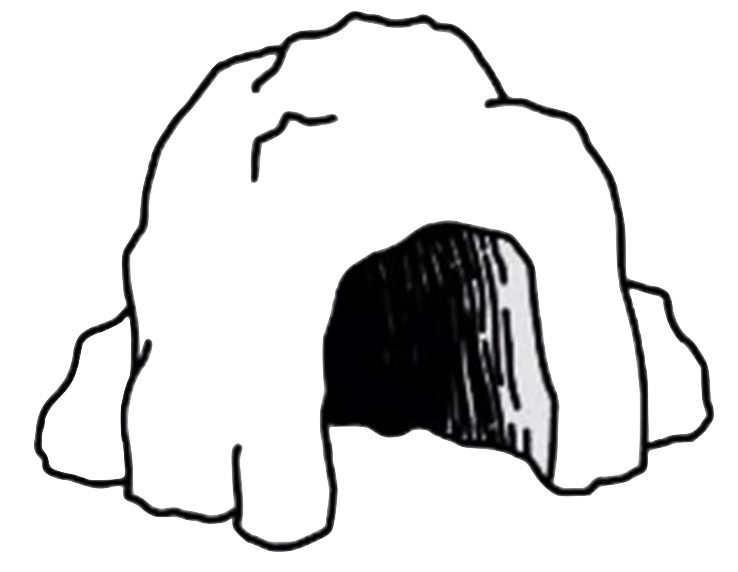
\includegraphics[width=4cm]{Concave.png}
    \end{figure}

\end{frame}

\begin{frame}
    \frametitle{Convexity and Concavity}
    Results/Theorem \& Comment\\
    \vspace{1em}
    1. Let $f:I\rightarrow\mathbb{R}$ be strictly convex on $I$ and differentiable at $a,b\in I$. Then:
    \begin{enumerate}
        \item[i] For any $h>0(h<0)$ such that $a+h\in I$, the graph of $f$ over the interval $(a,a+h)$ lies below the secant line through the
            points $(a,f(a))$ and $(a+h, f(a+h))$
        \item[ii] The graph of $f$ over all $I$ lies above the tangent line through the point $(a, f(a))$
        \item[iii] If $a<b$, then $f~'(a)<f~'(b)$
    \end{enumerate}
    \vspace{1em}
    \textcolor{red}{Draw some pictures to visualize these results!}
\end{frame}

\begin{frame}
    \frametitle{Convexity and Concavity}
    Results/Theorem \& Comment\\
    \vspace{1em}
    2. A function $f:I\rightarrow\mathbb{R}$($I$ is an interval) is convex if and only if
    \begin{equation*}
        \underset{t\in(0,1)}{\forall}\ \underset{x,y\in I}{\forall}\text{ with } x<y, f(tx+(1-t)y)\leq tf(x)+(1-t)f(y)
    \end{equation*}\\

    \textcolor{red}{Draw some pictures to visualize these results!}

    \vspace{2em}
    3. Let $I$ be an interval, $f:I\rightarrow\mathbb{R}$ differentiable and $f~'$ strictly increasing. If $a, b\in I$, $a<b$ and
    $f(a)=f(b)$, then
    \begin{equation*}
        f(x)<f(a)=f(b)\text{ for all }x\in(a,b)
    \end{equation*}

\end{frame}
\begin{frame}
    \frametitle{Inflection Point}
    Definition: inflection point is a point on a smooth plane curve at which the curvature changes sign. In particular, in the case of the graph of a function, it is a point where the function changes from being concave (concave downward) to convex (concave upward), or vice versa.
    \begin{figure}[htbp]
        \centering
        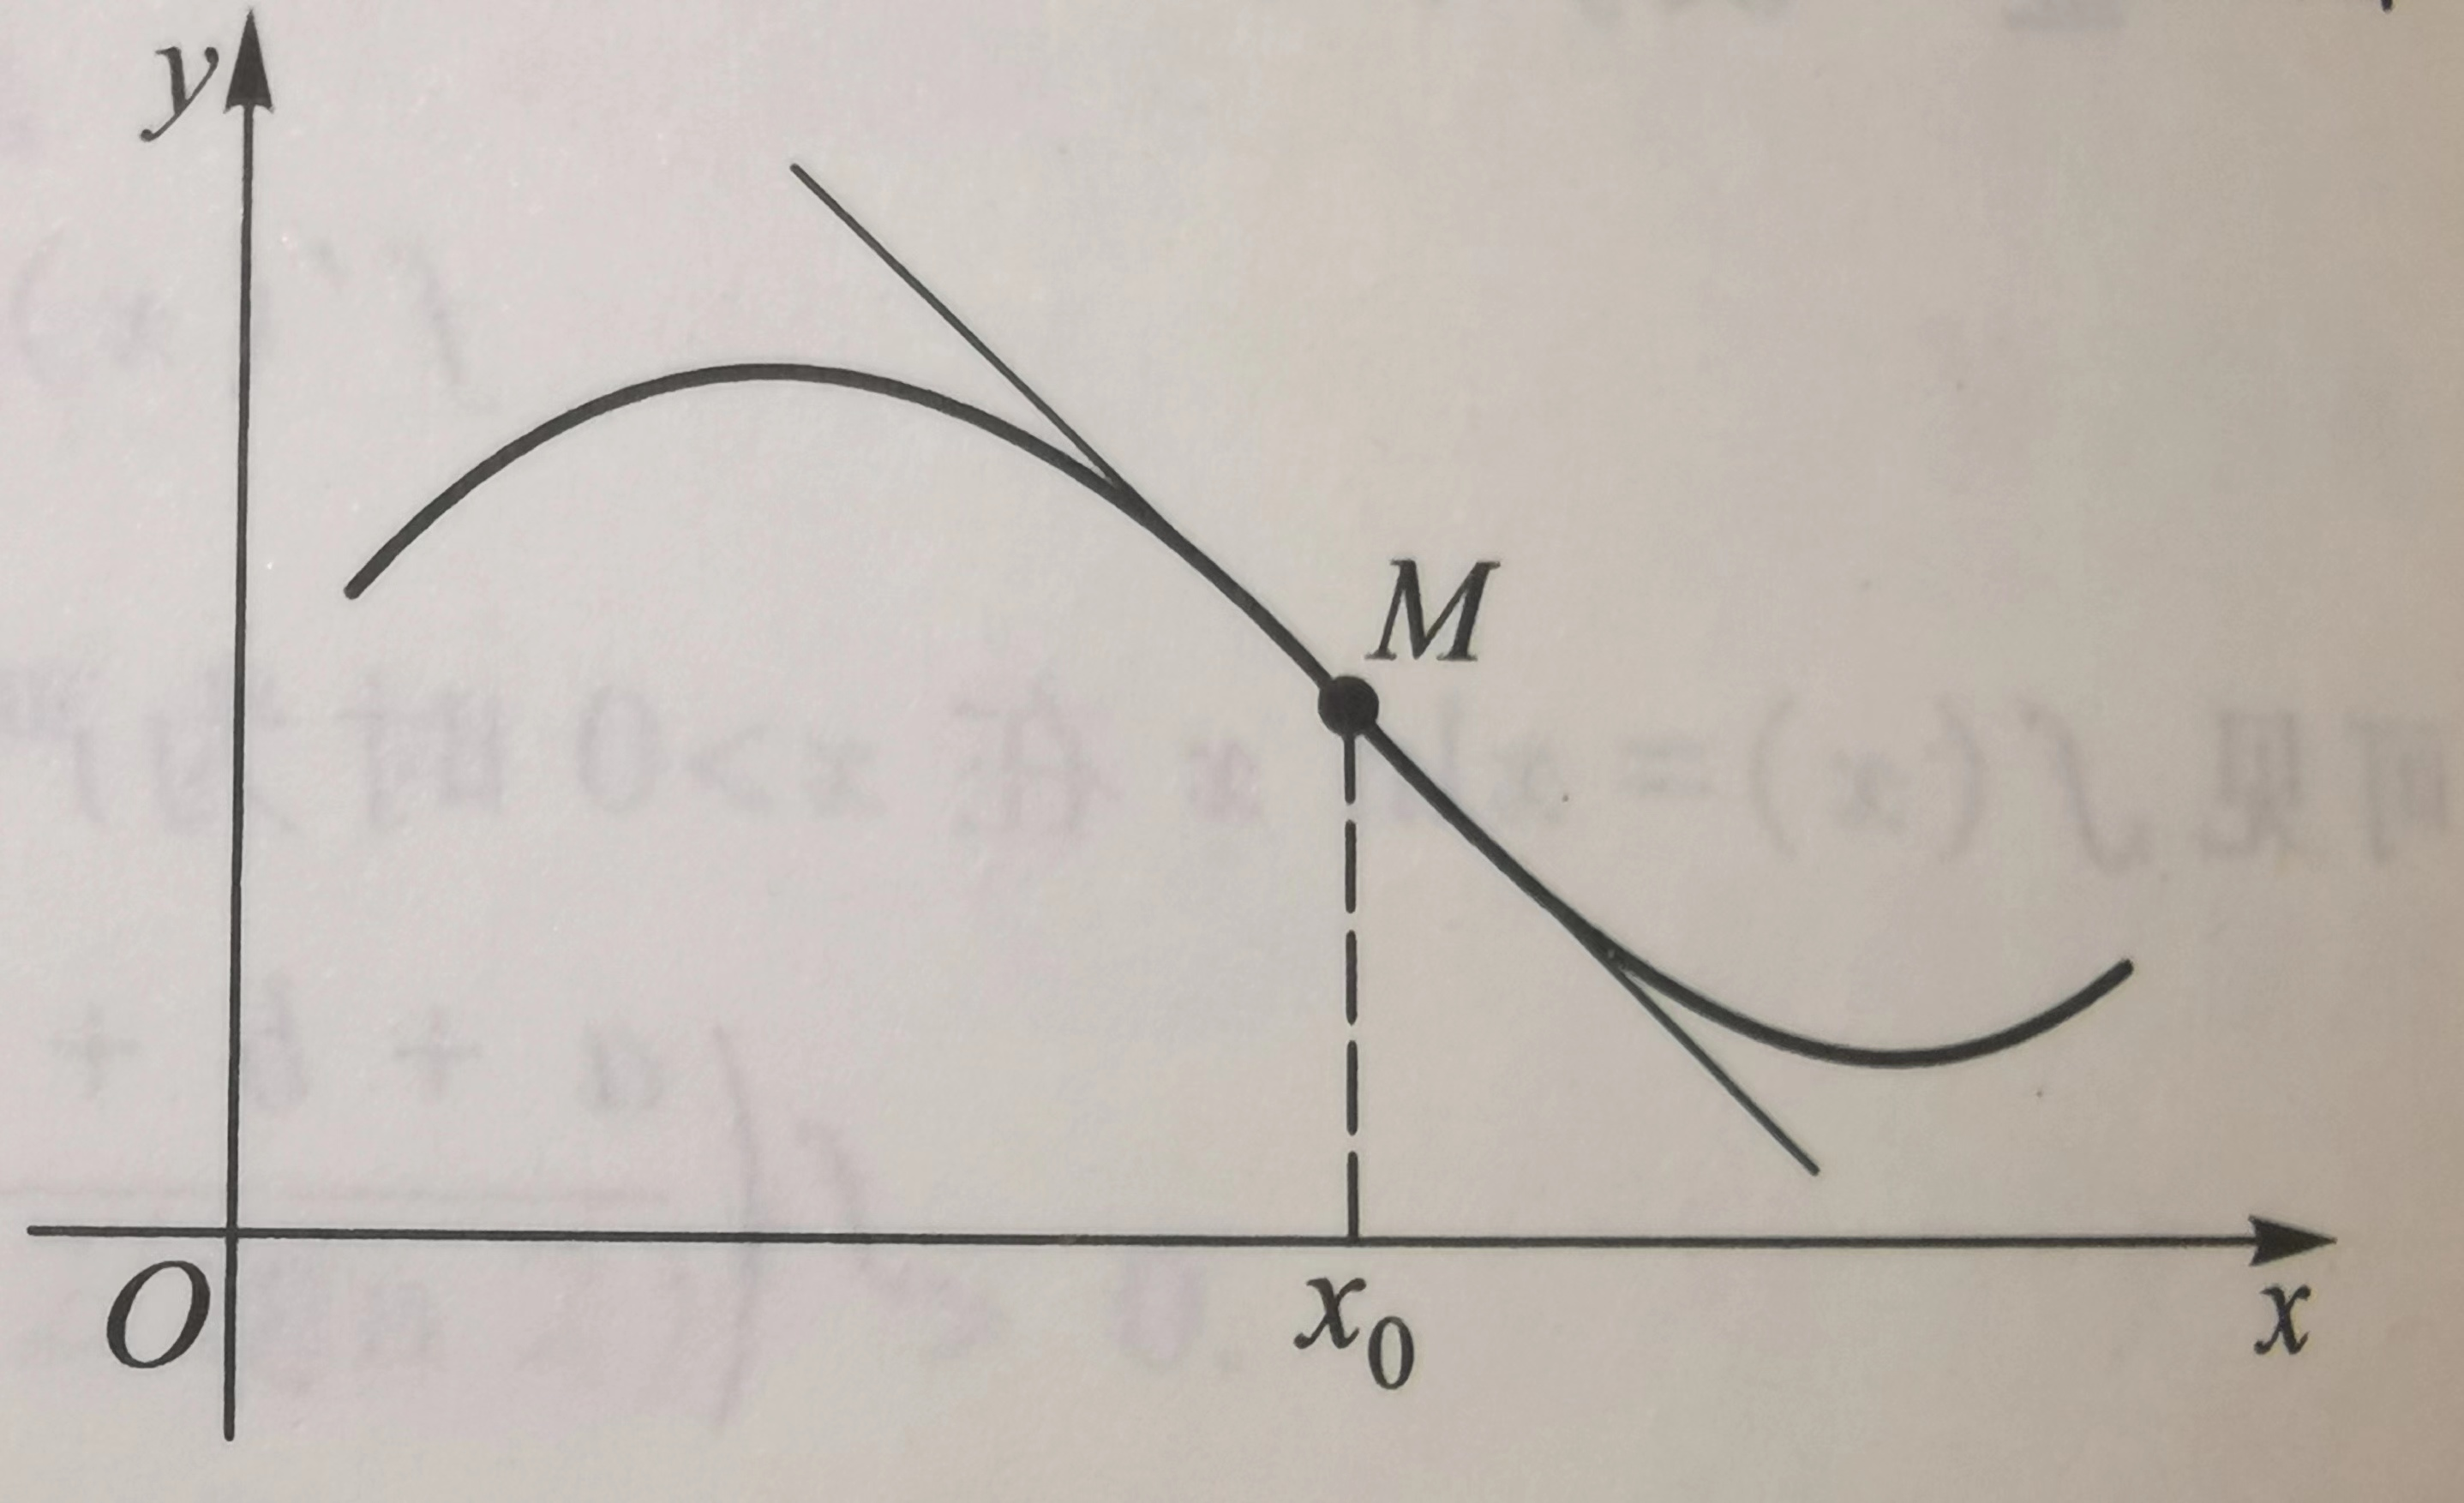
\includegraphics[width=8cm]{inflection.jpg}
    \end{figure}
\end{frame}
\begin{frame}
    \frametitle{Exercise}
    1. This exercise will show why convexity is useful.
    \begin{enumerate}
        \item[i]    Let $f$ be a convex function on $[a,b]$. Prove that
            \begin{equation*}
                f(\sum^n_{i=1}\lambda_i x_i)\leq \sum^n_{i=1}\lambda_i f(x_i),\ x_i\in[a,b],\ \sum^n_{i=1}\lambda_i=1,\ \lambda_i>0
            \end{equation*}
            This inequality is known as \textbf{Jensen's Inequality}(for discrete measure.)
        \item[ii] Show that
            \begin{equation*}
                \prod^n_{i=1} a_i^{\lambda_i}\leq \sum^n_{i=1}\lambda_i a_i,\ a_i\geq 0,\ \sum^n_{i=1}\lambda_i=1,\ \lambda_i>0.
            \end{equation*}
            This is the inequality you will encounter in your assignment.
    \end{enumerate}
\end{frame}

\begin{frame}
    \frametitle{Exercise}
    2. Let $f:[0,1]\rightarrow\mathbb{R}$ be a continuous function. Prove that if $f$ satisfies
    \begin{equation*}
        f(\frac{x_1+x_2}{2})\leq \frac{1}{2}(f(x_1)+f(x_2))
    \end{equation*}
    , where $x_1,x_2\leq[0,1]$, then $f$ is convex.
\end{frame}

\begin{frame}
    \frametitle{Exercise}
    3. Left f be a convex function, f:[a,b]$\rightarrow\mathbb{R}$. If there exists c$\in$(a,b), f(a)=f(b)=f(c), prove that f is a constant function.
\end{frame}
\begin{frame}
    \frametitle{Exercise}
    4. Let $f$ be a continuous convex real function on $[a,b]$. Show that $f$ either has one local minimum or infinitely many local minimums on $[a,b]$.
\end{frame}
\begin{frame}
    \frametitle{Exercise}
    5. f(x) is a concave function on (a,b), and it is not constant. Prove that f(x) can't attain its maximum on (a,b).
\end{frame}
\begin{frame}
    \frametitle{Exercise}
    6. (Darboux Theorem)
    If f is differentiable on [a,b], prove that f$'$ can fetch all values between f$'$(a) and f$'$(b).
\end{frame}
\begin{frame}
    \begin{figure}[htbp]
        \centering
        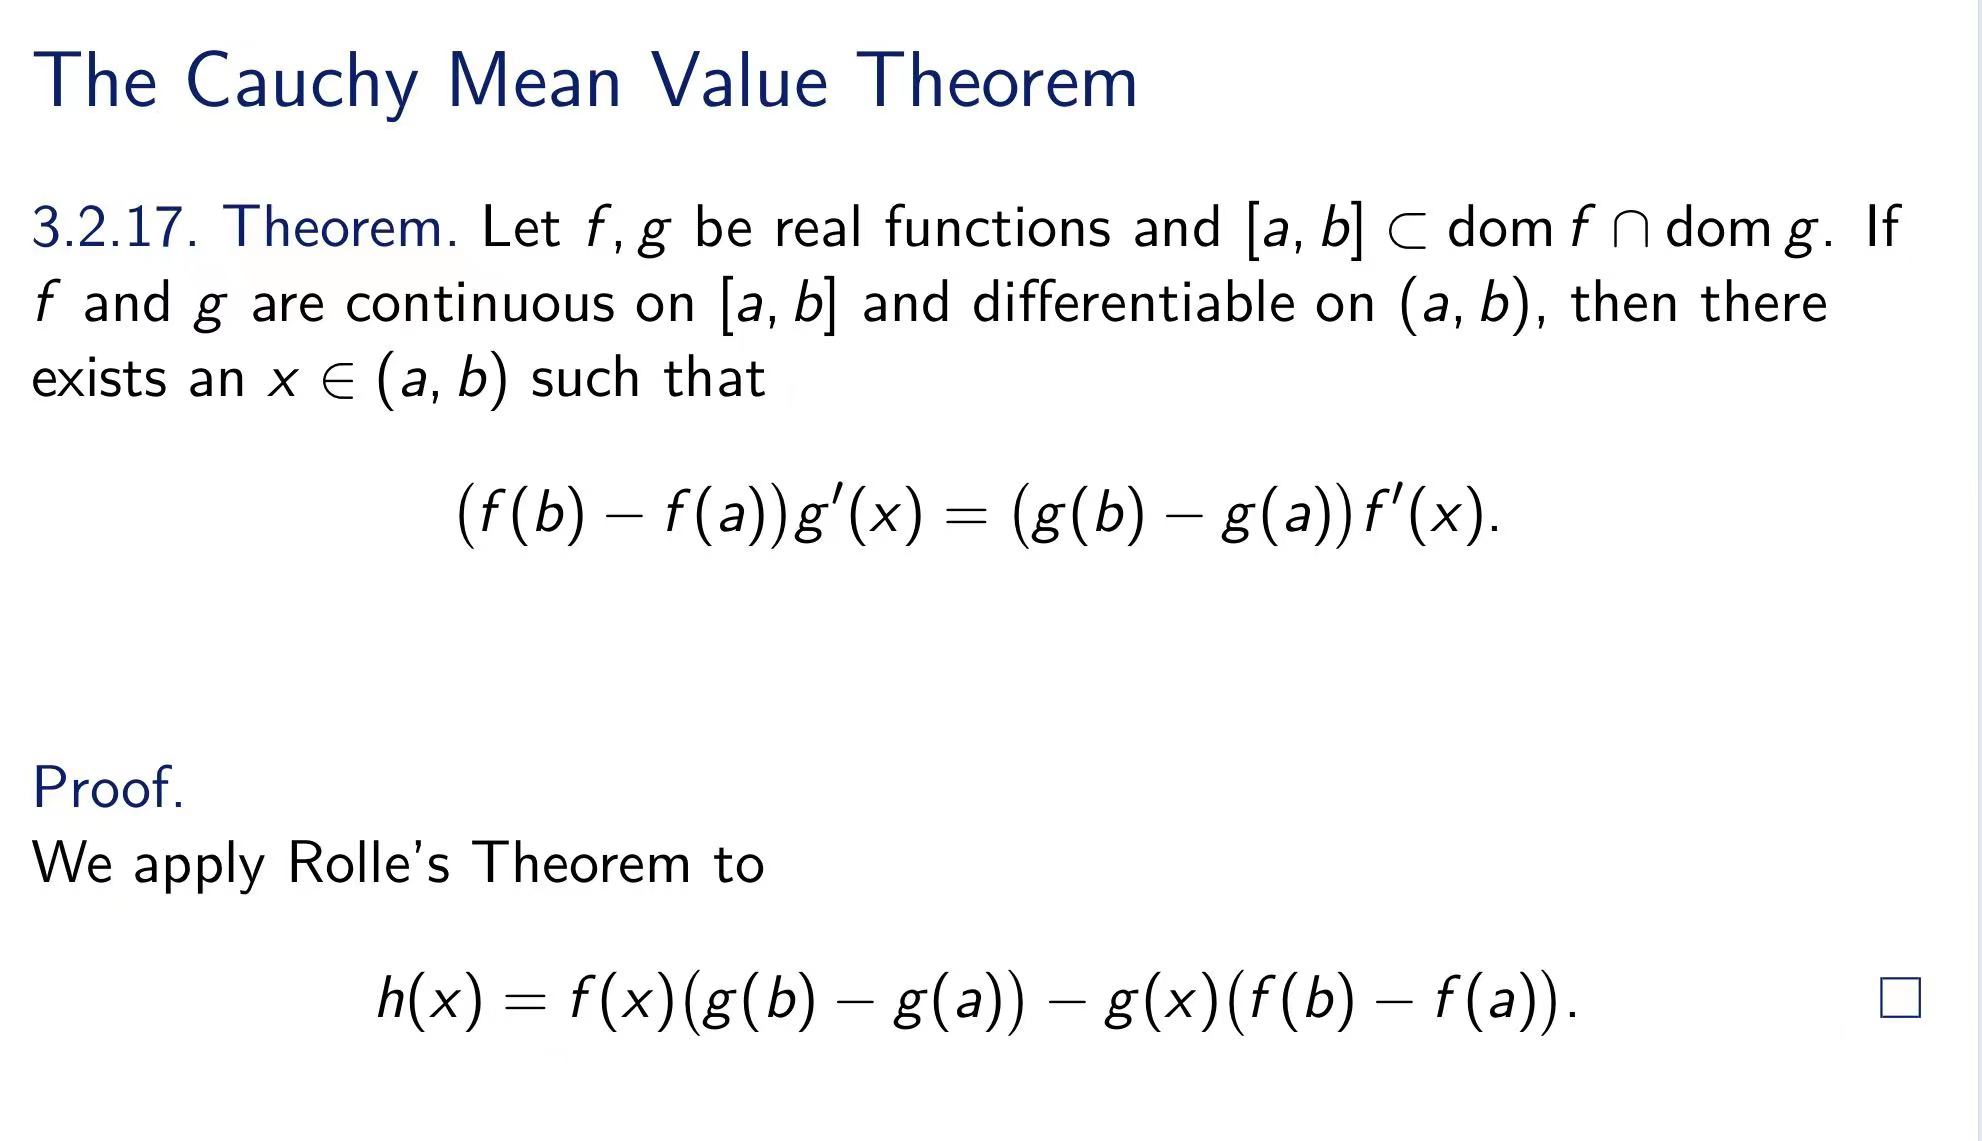
\includegraphics[width=12cm]{cauchy.jpg}
    \end{figure}
\end{frame}

\begin{frame}
    \frametitle{Exercise}
    7. Function f is continuous on [a,b], and differentiable on (a,b), prove that there exists $\xi\in(a,b)$, such that:
    \begin{equation*}
        f(b)-f(a)=\xi \ln\frac{b}{a}f'(\xi)
    \end{equation*}
\end{frame}

\begin{frame}
    \frametitle{Exercise}
    8. Prove that if f is differentiable on interval [a,b], and ab>0, then there exists a $\xi\in(a,b)$,such that:
    \begin{equation*}
        \frac{af(b)-b(a)}{a-b}=f(\xi)-\xi f'(\xi)
    \end{equation*}
\end{frame}

\begin{frame}
    9. Function f and g are differentiable on interval (a,b).
    \begin{center}
        F(x)=f(x)g$'$(x)-f$'$(x)g(x)
    \end{center}
    Prove that if F(x)>0 on (a,b), there must exist a solution for g(x)=0 between two different solutions for f(x)=0.
\end{frame}

\begin{frame}
    10. f(x) is differentiable on (a,b), prove that there is a solution for f(x)+f'(x)=0 between two solutions for f(x)=0 on (a,b).
\end{frame}

\begin{frame}
    11. f(x) is continuous on [0,1] and differentiable on(a,b), and f(0)=f(1)=0. Assume there exists $t_{0}\in (0,1)$, f($t_{0}$)=$\alpha$. Prove that there exists $\xi\in(0,1)$, such that $f'(\xi)=\alpha$.
\end{frame}

\begin{frame}
    \begin{figure}[htbp]
        \centering
        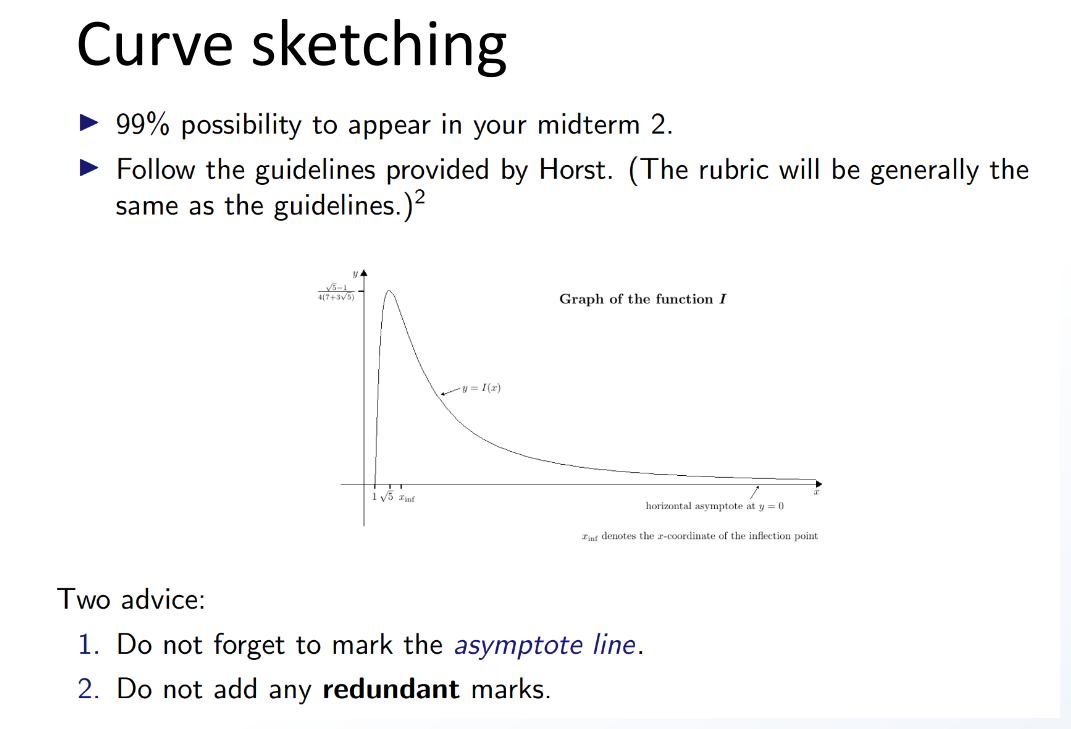
\includegraphics[width=12cm]{sketching.png}
    \end{figure}
\end{frame}

\begin{frame}
    \frametitle{Reference}
    \begin{itemize}
        \item Exercises from 2021VV186-Niyinchen.
        \item Graph from 2021VV186-Huangyue
    \end{itemize}
\end{frame}
\begin{frame}
    \frametitle{End}
    \centering
    \LARGE{Thanks!}


\end{frame}
\end{document}